\definecolor{r1}{RGB}{86,16,16};
\definecolor{r2}{RGB}{151,28,28};
\definecolor{r3}{RGB}{214,39,40};
\definecolor{r4}{RGB}{227,104,104};
\definecolor{r5}{RGB}{239,169,169};
\definecolor{b1}{RGB}{11,43,65};
\definecolor{b2}{RGB}{22,86,131};
\definecolor{b3}{RGB}{31,119,180};
\definecolor{b4}{RGB}{59,154,222};
\definecolor{b5}{RGB}{124,188,233};
\definecolor{g1}{RGB}{16,60,16};
\definecolor{g2}{RGB}{33,120,33};
\definecolor{g3}{RGB}{49,180,49};
\definecolor{g4}{RGB}{95,211,95};
\definecolor{g5}{RGB}{135,222,135};
\definecolor{p1}{RGB}{39,23,53};
\definecolor{p2}{RGB}{77,47,106};
\definecolor{p3}{RGB}{116,70,160};
\definecolor{p4}{RGB}{148,103,189};
\definecolor{p5}{RGB}{179,149,208};
\definecolor{tab_orange}{RGB}{255,127,14};
\definecolor{tab_blue}{RGB}{31, 119, 180};
\definecolor{mixed_color}{RGB}{143, 123, 97}
\definecolor{tab_brown}{RGB}{140,86,75};


\begin{tikzpicture}

\node at (0.3,12.7) {{\fontfamily{phv}\scalebox{1}{\fontsize{8pt}{0pt}\selectfont{A}}}};

\node at (3.1,12.7) {{\fontfamily{phv}\scalebox{1}{\fontsize{7pt}{0pt}\selectfont \parbox{4.5cm} {\hyphenpenalty=10000\exhyphenpenalty=10000\raggedright
Proportion of diagnoses in patients
}}}};
\node[inner sep=0pt] (russell) at (2.4,9.7) {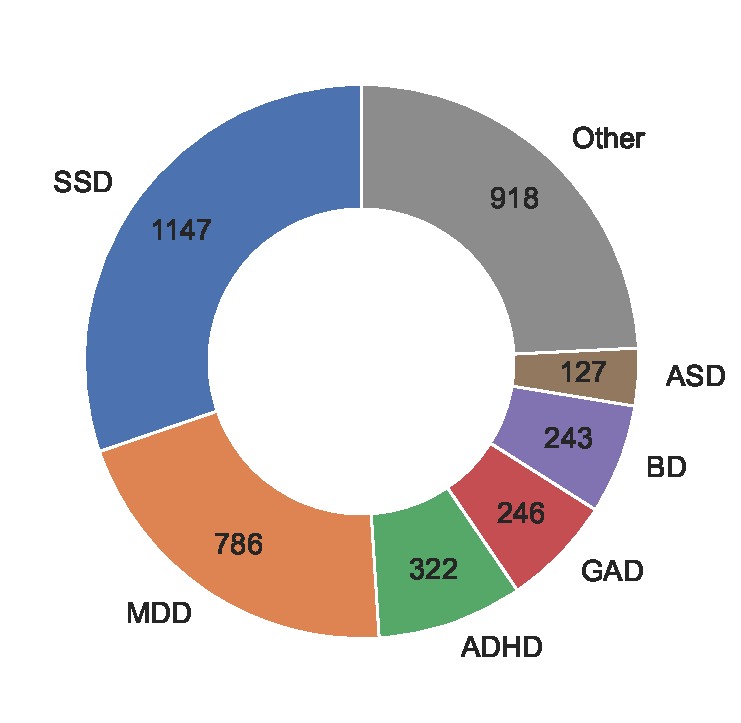
\includegraphics[width=0.25\textwidth]{figs3.1.pdf}};












\node at (5.7,12.7) {{\fontfamily{phv}\scalebox{1}{\fontsize{8pt}{0pt}\selectfont{B}}}};

\node at (8.5,12.7) {{\fontfamily{phv}\scalebox{1}{\fontsize{7pt}{0pt}\selectfont \parbox{4.5cm} {\hyphenpenalty=10000\exhyphenpenalty=10000\raggedright
Age distribution across diagnoses
}}}};
\node[inner sep=0pt] (russell) at (10.9,9.6) {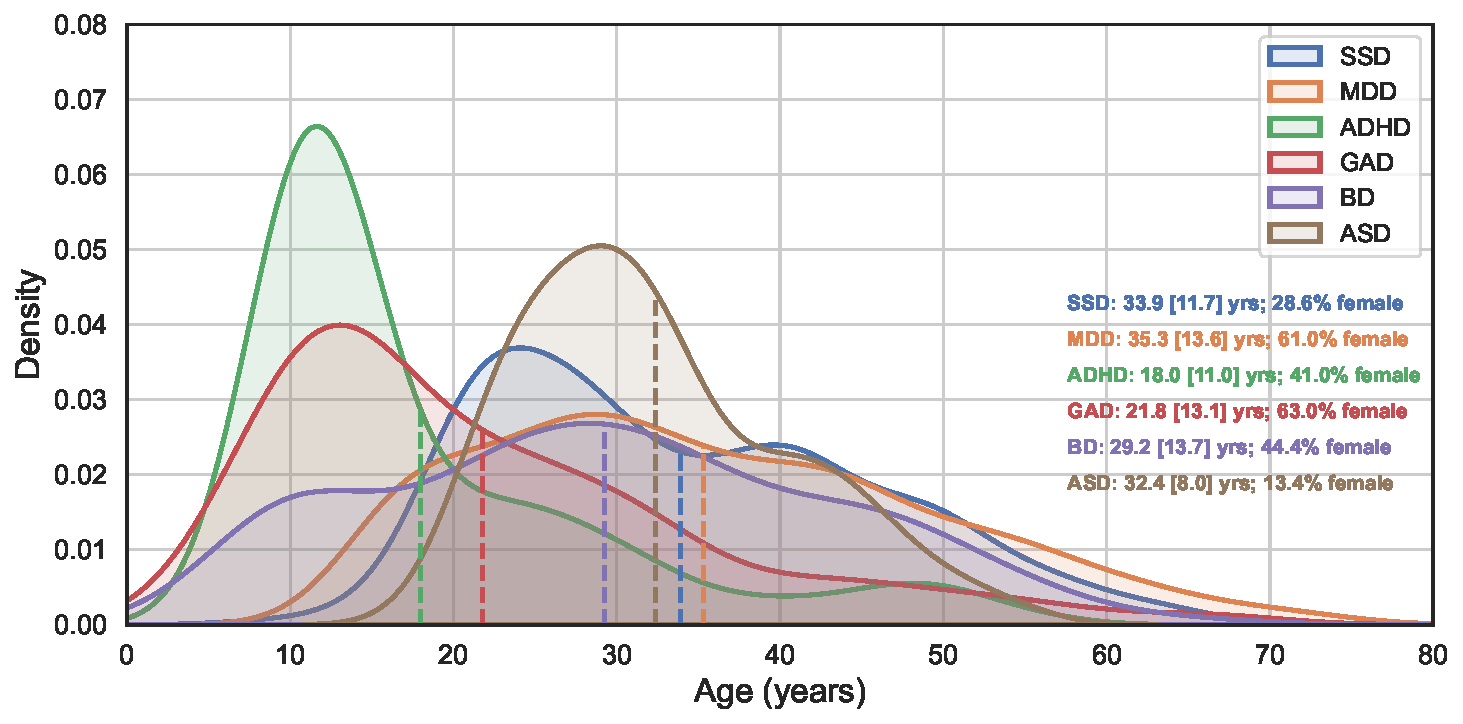
\includegraphics[width=0.50\textwidth]{figs3.3.pdf}};


\node at (0.3,6.4) {{\fontfamily{phv}\scalebox{1}{\fontsize{8pt}{0pt}\selectfont{C}}}};

\node at (3.1,6.4) {{\fontfamily{phv}\scalebox{1}{\fontsize{7pt}{0pt}\selectfont \parbox{4.5cm} {\hyphenpenalty=10000\exhyphenpenalty=10000\raggedright
Proportion of data modalities 
}}}};
\node[inner sep=0pt] (russell) at (2.18,3.3) {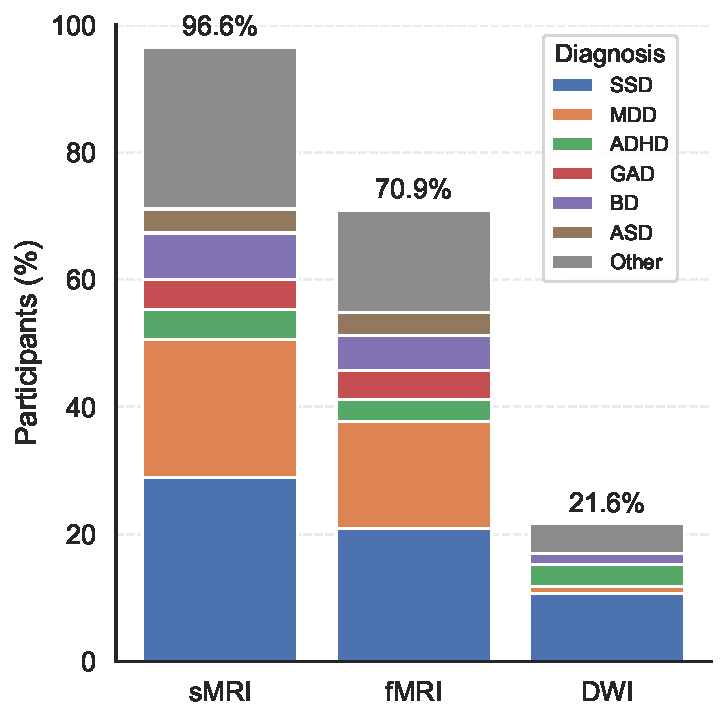
\includegraphics[width=0.25\textwidth]{fig3.4.pdf}};


\node[inner sep=0pt] (russell) at (10.7,2.9) {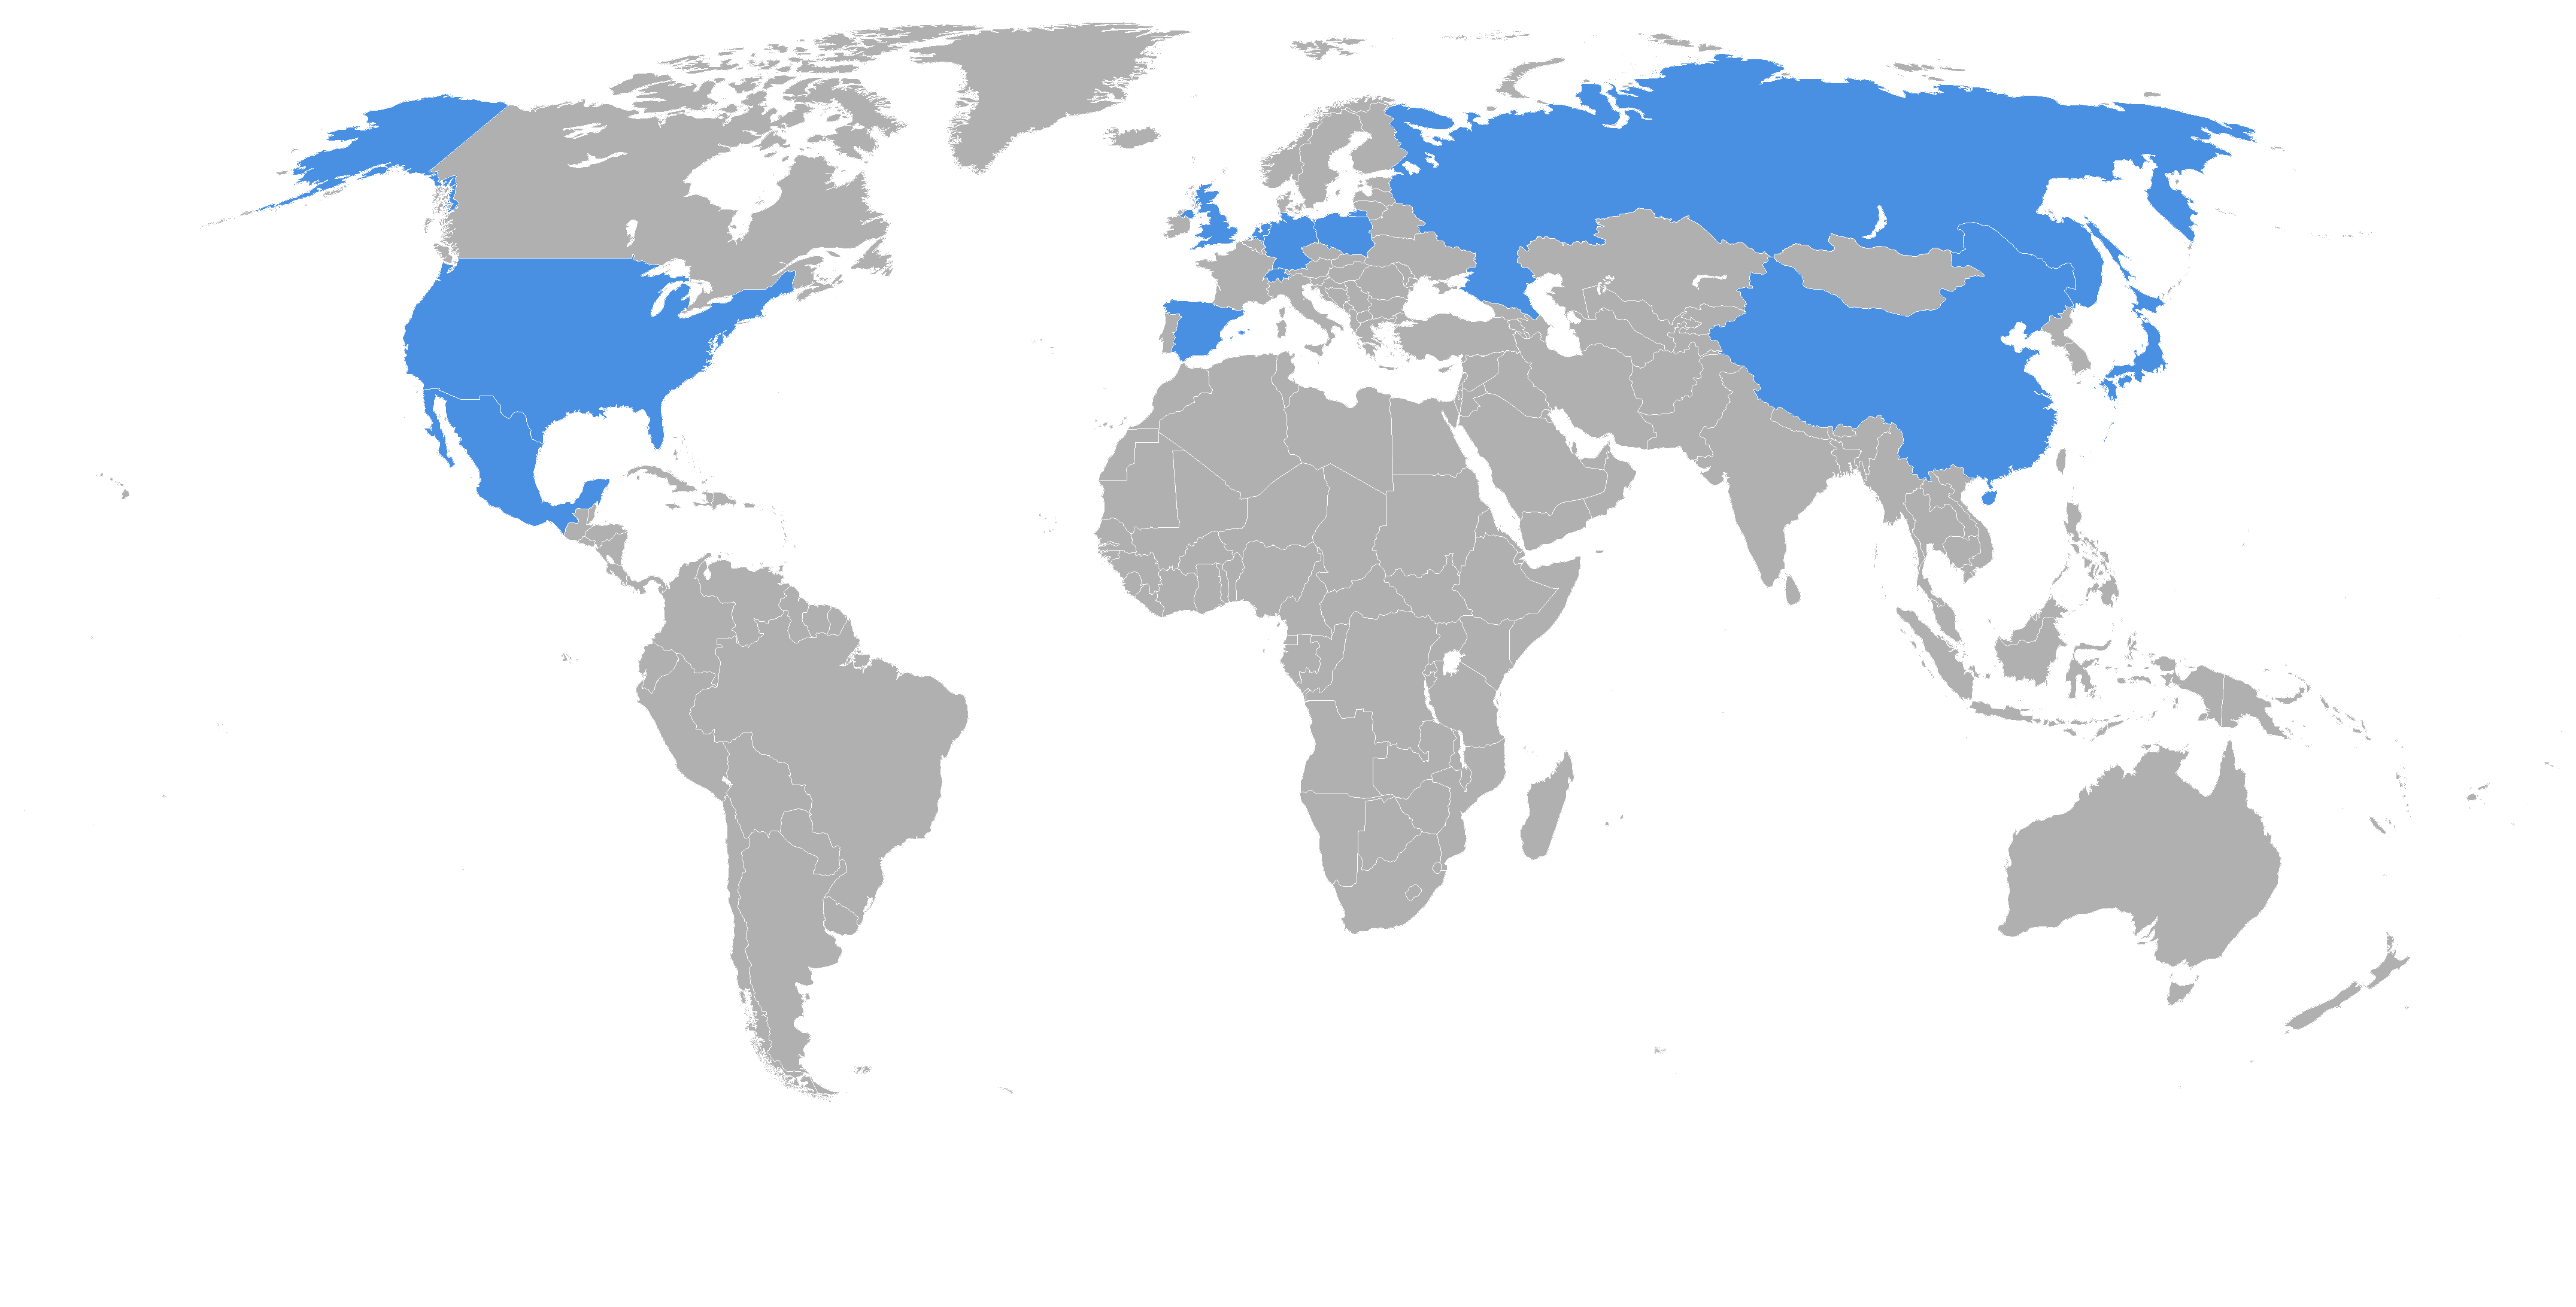
\includegraphics[width=0.59\textwidth]{world.pdf}};


\node at (5.7,6.4) {{\fontfamily{phv}\scalebox{1}{\fontsize{8pt}{0pt}\selectfont{D}}}};

\node at (8.5,6.4) {{\fontfamily{phv}\scalebox{1}{\fontsize{7pt}{0pt}\selectfont \parbox{4.5cm} {\hyphenpenalty=10000\exhyphenpenalty=10000\raggedright
Geographical distribution of samples 
}}}};

\node at (7.1,4.5) {{\fontfamily{phv}\scalebox{1}{\fontsize{5pt}{0pt}\selectfont {USA (19)}}}};
\node at (9.7,4.8) {{\fontfamily{phv}\scalebox{1}{\fontsize{5pt}{0pt}\selectfont {NLD (3)}}}};
\node at (9.7,4.6) {{\fontfamily{phv}\scalebox{1}{\fontsize{5pt}{0pt}\selectfont {GBR (4)}}}};
\node at (9.7,4.4) {{\fontfamily{phv}\scalebox{1}{\fontsize{5pt}{0pt}\selectfont {CHE (1)}}}};
\node at (9.7,4.2) {{\fontfamily{phv}\scalebox{1}{\fontsize{5pt}{0pt}\selectfont {ESP (1)}}}};
\node at (13.8,4.3) {{\fontfamily{phv}\scalebox{1}{\fontsize{5pt}{0pt}\selectfont {CHN (1)}}}};
\node at (9.7,5) {{\fontfamily{phv}\scalebox{1}{\fontsize{5pt}{0pt}\selectfont {DEU (1)}}}};
\node at (13.1,5.3) {{\fontfamily{phv}\scalebox{1}{\fontsize{5pt}{0pt}\selectfont {RUS (1)}}}};
\node at (15.3,4.1) {{\fontfamily{phv}\scalebox{1}{\fontsize{5pt}{0pt}\selectfont {JPN (1)}}}};
\node at (6.5,3.4) {{\fontfamily{phv}\scalebox{1}{\fontsize{5pt}{0pt}\selectfont {MEX (1)}}}};
\node at (9.7,5.2) {{\fontfamily{phv}\scalebox{1}{\fontsize{5pt}{0pt}\selectfont {POL (1)}}}};





\end{tikzpicture}